% Book 3, Year 1, chapter 29 -- the relational model, relational algebra and SQL.
% Provenance (never printed): sources/book3/BRIEFS.md, chapter 29.
% ledger: b1:codd-1970, b1:chen-1976, b1:sqlite-fk
\chapter{The Relational Model, Relational Algebra and SQL}\label{ch:b1:relational-model}

The town's library wants to write to the members who have never borrowed a book of poetry. Three colleagues each write
a query. The first takes all the members and removes those who borrowed poetry; the second keeps each member for whom
no poetry loan exists; the third joins members to poetry loans and keeps those left without a partner. All three print
28. Is that luck, or are they the same question? To answer, a query must be more than text: it must be a mathematical
object, with laws that say when two of them are equal. That object is \omterm{def:b1:relational-model:algebra}{relational algebra}, and this chapter reads SQL
through it. It ends with the other half of the work, designing the tables in the first place.

\begin{recall}
A \omterm{def:b1:relational-model:relation}{relation} between sets is a subset of their \omterm{def:b1:relational-model:join}{Cartesian product} (mathematics book, Year 1). The second book used the
town's tables in SQLite with \code{SELECT}, joins and keys; \omterm{def:b1:propositional-logic:valuation}{valuations} of formulas are in
\cref{def:b1:propositional-logic:valuation}. Every query here runs on the town's \code{books}, \code{members} and
\code{loans}, through the series' SQL runner, which prints each statement after \code{sql>}.
\end{recall}

\section{Relations, keys and integrity constraints}\label{sec:b1:relational-model:relations}

\begin{definition}[Relation schema, attribute, domain]\label{def:b1:relational-model:schema}
A \emph{relation schema}\index{relation schema} $R(A_1, \dots, A_n)$ is a name and a finite set of
\emph{attributes}\index{attribute (of a relation)} $A_1, \dots, A_n$, each with a \emph{domain}\index{domain (of an
attribute)} $D_i$, the set of values it may take.
\end{definition}

\begin{definition}[Tuple, relation]\label{def:b1:relational-model:relation}
A \emph{tuple}\index{tuple (of a relation)} over the schema gives each attribute $A_i$ a value in $D_i$. A
\emph{relation}\index{relation (database)} over the schema (an instance) is a finite set of tuples: a subset of $D_1
\times \dots \times D_n$, the \omterm{def:b1:relational-model:schema}{attributes} naming the positions.
\end{definition}

A \omterm{def:b1:relational-model:relation}{relation} is a set: its \omterm{def:b1:relational-model:relation}{tuples} have no order and no duplicates. A table in a database is close to that, but not quite,
and the differences (order, duplicates, NULL) are where SQL surprises.

\begin{definition}[Superkey, candidate key, primary key, foreign key]\label{def:b1:relational-model:keys}
A \emph{superkey}\index{superkey} of a schema is a set of \omterm{def:b1:relational-model:schema}{attributes} on which no two \omterm{def:b1:relational-model:relation}{tuples} of any allowed instance
agree. A \emph{candidate key}\index{candidate key} is a superkey none of whose proper subsets is one. The \emph{primary
key}\index{primary key} is the candidate key chosen to identify \omterm{def:b1:relational-model:relation}{tuples}. A \emph{foreign key}\index{foreign key} of $R$ is a
set of \omterm{def:b1:relational-model:schema}{attributes} whose values must appear as the primary key of some \omterm{def:b1:relational-model:relation}{tuple} of another \omterm{def:b1:relational-model:relation}{relation} $S$: it
\emph{references} $S$.
\end{definition}

\begin{definition}[Integrity constraint, referential integrity]\label{def:b1:relational-model:integrity}
An \emph{integrity constraint}\index{integrity constraint} is a condition that every instance of a database must satisfy:
a key, a NOT NULL, a CHECK on the values of a \omterm{def:b1:relational-model:relation}{tuple}. \emph{Referential integrity}\index{referential integrity} is the
constraint that every \omterm{def:b1:relational-model:keys}{foreign key} value appears in the \omterm{def:b1:relational-model:relation}{relation} it references.
\end{definition}

\begin{definition}[Null marker]\label{def:b1:relational-model:null}
The \emph{null marker}\index{null marker} \code{NULL} stands in a \omterm{def:b1:relational-model:relation}{tuple} for a value that is missing or unknown. It is not a
value of the \omterm{def:b1:relational-model:schema}{domain}: it equals nothing, not even itself.
\end{definition}

The library's own schema, designed in \cref{sec:b1:relational-model:er}, writes each of these in SQL's data definition
language: \code{PRIMARY KEY}, \code{UNIQUE} (another \omterm{def:b1:relational-model:keys}{candidate key}), \code{REFERENCES} (a \omterm{def:b1:relational-model:keys}{foreign key}), \code{NOT NULL}
and \code{CHECK}.

\omcode{code/bachelor-1/29-relational-model/listings/schema.sql}{18}{27}{The table of loans and its
constraints}\label{lst:b1:relational-model:schema}

\omoutput{code/bachelor-1/29-relational-model/outputs/constraints.txt}{Four statements accepted (five rows), then six
refused, one per constraint; the last would leave a loan pointing at nothing.}\label{out:b1:relational-model:constraints}

The database is the guardian of its own consistency: no program can store a loan of a book that does not exist, however
it is written. One trap is SQLite's alone: for compatibility with old databases, it checks \omterm{def:b1:relational-model:keys}{foreign keys} only after
\code{PRAGMA foreign_keys = ON}, on each connection, and the series' runner sends it.

\omoutput{code/bachelor-1/29-relational-model/outputs/fk_off.txt}{With the check off, a loan of book 999 by member 10, who
do not exist, is accepted; \code{foreign_key_check} finds it afterwards.}\label{out:b1:relational-model:fk-off}

\begin{omfigure}
\begin{tikzpicture}[font=\small]
\node[inner sep=0pt, anchor=north west] (bk) at (0,0) {\begin{tabular}{|c|l|l|l|}
\multicolumn{4}{l}{\code{books}} \\ \hline
\underline{\textbf{book\_id}} & \textbf{title} & \textbf{author} & \textbf{genre} \\ \hline
1 & The Silent Code & Fatou Dalewell & mystery \\
2 & The Paper Forest & Zoe Stoneton & sport \\
\dots & \dots & \dots & \dots \\ \hline
\end{tabular}};
\node[inner sep=0pt, anchor=north west] (ln) at (0,-3.0) {\begin{tabular}{|c|c|c|c|c|}
\multicolumn{5}{l}{\code{loans}} \\ \hline
\underline{\textbf{loan\_id}} & \textbf{book\_id} & \textbf{member\_id} & \textbf{out\_date} &
\textbf{return\_date} \\ \hline
1 & 59 & 41 & 2025-01-01 & 2025-01-03 \\
3 & 28 & 58 & 2025-01-01 & NULL \\ \hline
\end{tabular}};
\draw[->, thick, omThm] ($(ln.north west)+(2.25,-0.45)$) to[out=100, in=-80]
  node[right, font=\scriptsize] {foreign key} ($(bk.south west)+(0.65,0)$);
\node[anchor=west, font=\scriptsize, align=left] at ($(bk.east)+(0.4,0.35)$) {the schema: a name\\ and attributes};
\node[anchor=west, font=\scriptsize, align=left] at ($(bk.east)+(0.4,-0.55)$) {the tuples: a set,\\ in no order};
\end{tikzpicture}
\par\smallskip{\small Two \omterm{def:b1:relational-model:relation}{relations} of the town, with some of their \omterm{def:b1:relational-model:schema}{attributes} (\code{books} also has a year
and a number of pages, \code{loans} a due date). The \omterm{def:b1:relational-model:keys}{primary keys} are underlined; each value of \code{loans.book_id} must
be the key of a \omterm{def:b1:relational-model:relation}{tuple} of \code{books}. A NULL return date means the book is still out.}
\end{omfigure}

\omimg{book3/ai/b1-relational-model-card-catalogue.jpg}{0.5\linewidth}{A library's card catalogue was a \omterm{def:b1:relational-model:relation}{relation} on
paper: one card per book, the same fields on every card, and drawers kept in the order of one attribute, so that a
search by another attribute meant reading every card.}

\section{Relational algebra}\label{sec:b1:relational-model:algebra}

\begin{definition}[Relational algebra]\label{def:b1:relational-model:algebra}
\emph{Relational algebra}\index{relational algebra} is the set of operators that take \omterm{def:b1:relational-model:relation}{relations} and return a \omterm{def:b1:relational-model:relation}{relation},
and of the expressions built from them and from named \omterm{def:b1:relational-model:relation}{relations}. A query is an expression.
\end{definition}

\begin{definition}[Selection, projection, renaming]\label{def:b1:relational-model:selection}
For a \omterm{def:b1:relational-model:relation}{relation} $r$ over \omterm{def:b1:relational-model:schema}{attributes} $U$: the \emph{selection}\index{selection (relational algebra)} $\sigma_c(r)$ is the set
of \omterm{def:b1:relational-model:relation}{tuples} of $r$ that satisfy the condition $c$; the \emph{projection}\index{projection (relational algebra)}
$\pi_X(r)$, for $X \subseteq U$, is the set of the restrictions $t[X]$ of the \omterm{def:b1:relational-model:relation}{tuples} of $r$ to $X$; the
\emph{renaming}\index{renaming (relational algebra)} $\rho_{B \leftarrow A}(r)$ is $r$ with the attribute $A$ called $B$.
\end{definition}

The set operations $r \cup s$ and $r - s$ apply to \omterm{def:b1:relational-model:relation}{relations} over the same \omterm{def:b1:relational-model:schema}{attributes}.

\begin{definition}[Cartesian product, natural join, theta join, left outer join]\label{def:b1:relational-model:join}
For $r$ over $U$ and $s$ over $V$:
the \emph{Cartesian product}\index{Cartesian product (of relations)} $r \times s$, for disjoint $U$ and $V$, is the set
of the \omterm{def:b1:relational-model:relation}{tuples} $t \cup u$, $t \in r$, $u \in s$. The \emph{natural join}\index{natural join} $r \bowtie s$ is the set of the
\omterm{def:b1:relational-model:relation}{tuples} $w$ over $U \cup V$ with $w[U] \in r$ and $w[V] \in s$: the pairs that agree on the common \omterm{def:b1:relational-model:schema}{attributes}, each kept
once. A \emph{theta join}\index{theta join} is $r \bowtie_c s = \sigma_c(r \times s)$. The \emph{left outer
join}\index{left outer join} keeps, in addition, each \omterm{def:b1:relational-model:relation}{tuple} of $r$ that matches nothing, its \omterm{def:b1:relational-model:schema}{attributes} from $V - U$ set to
NULL.
\end{definition}

The \omterm{def:b1:relational-model:join}{natural join} is a product followed by a \omterm{def:b1:relational-model:selection}{selection} and a \omterm{def:b1:relational-model:selection}{projection}, and the intersection is $r \cap s = r - (r -
s)$: six operators, $\sigma$, $\pi$, $\rho$, $\cup$, $-$ and $\times$, are enough for the rest. The next one is the
algebra's ``for all''.

\begin{definition}[Division]\label{def:b1:relational-model:division}
For $r$ over $X \cup Y$ and $s$ over $Y$, with $X$ and $Y$ disjoint, the \emph{division}\index{division (relational
algebra)} $r \div s$ is the set of the \omterm{def:b1:relational-model:relation}{tuples} $x$ over $X$ such that $x \cup y \in r$ for every $y \in s$. It equals
$\pi_X(r) - \pi_X\big((\pi_X(r) \times s) - r\big)$: the candidates, minus those missing some pair.
\end{definition}

\omcode{code/bachelor-1/29-relational-model/listings/algebra.py}{23}{60}{\omterm{def:b1:relational-model:algebra}{Relational algebra} on Python sets: each operator
as its definition}\label{lst:b1:relational-model:algebra}

\omcode{code/bachelor-1/29-relational-model/listings/algebra_demo.py}{18}{28}{Three questions, as algebra on the
town's tables}\label{lst:b1:relational-model:demo}

\omoutput{code/bachelor-1/29-relational-model/outputs/algebra_demo.txt}{Each algebra answer compared with the SQL query
written next to it in the program.}\label{out:b1:relational-model:demo}

An algebra has laws. Two of them are the basis of every query optimiser.

\begin{proposition}[Selection laws]\label{prop:b1:relational-model:pushdown}
For \omterm{def:b1:relational-model:relation}{relations} $r, r'$ over $U$, $s$ over $V$, and conditions $c, c'$:
(i) $\sigma_c(\sigma_{c'}(r)) = \sigma_{c \wedge c'}(r)$;
(ii) $\sigma_c(r \cup r') = \sigma_c(r) \cup \sigma_c(r')$;
(iii) if $c$ mentions only \omterm{def:b1:relational-model:schema}{attributes} of $U$, then $\sigma_c(r \bowtie s) = \sigma_c(r) \bowtie s$.
\end{proposition}

\begin{proof}
(i) Both sides are the \omterm{def:b1:relational-model:relation}{tuples} of $r$ satisfying $c$ and $c'$. (ii) A \omterm{def:b1:relational-model:relation}{tuple} is on the left iff it is in $r$ or $r'$ and
satisfies $c$, which is the right. (iii) Let $w$ be over $U \cup V$. $w$ is on the left iff $w[U] \in r$, $w[V] \in s$ and
$w$ satisfies $c$. Since $c$ mentions only $U$, $w$ satisfies $c$ iff $w[U]$ does; so the condition reads $w[U] \in
\sigma_c(r)$ and $w[V] \in s$, the definition of the right side.
\end{proof}

The \omterm{def:b1:relational-model:join}{natural join} is also commutative and associative (\cref{exo:b1:relational-model:11}), so a query engine may reorder
joins. Pushing a \omterm{def:b1:relational-model:selection}{selection} below a join is what makes the reordering pay.

\omcode{code/bachelor-1/29-relational-model/listings/laws.py}{14}{24}{The laws on random \omterm{def:b1:relational-model:relation}{relations}}\label{lst:b1:relational-model:laws}

\omoutput{code/bachelor-1/29-relational-model/outputs/laws.txt}{The laws hold on 2000 random cases; on the town, the
pushed-down plan builds 49 \omterm{def:b1:relational-model:relation}{tuples} instead of 400.}\label{out:b1:relational-model:laws}

\begin{omfigure}
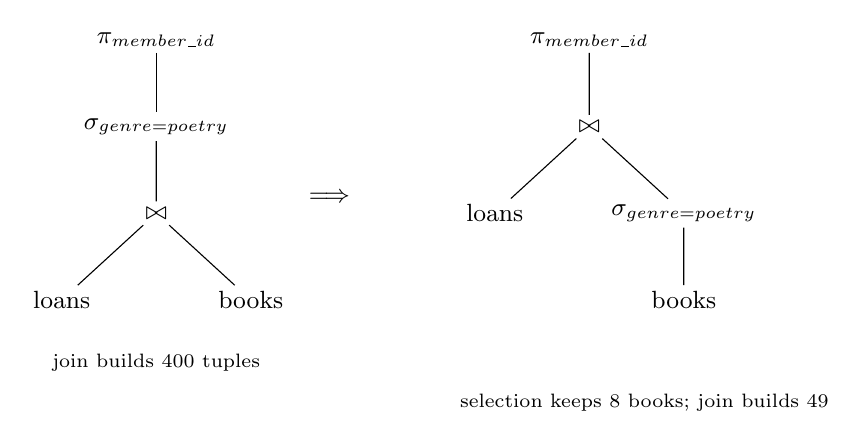
\begin{tikzpicture}[font=\small, level distance=11mm, sibling distance=24mm, every node/.style={inner sep=2pt}]
\node {$\pi_{\text{member\_id}}$}
  child {node {$\sigma_{\text{genre} = \text{poetry}}$}
    child {node {$\bowtie$}
      child {node {\code{loans}}} child {node {\code{books}}}}};
\node at (2.2,-2.0) {$\Longrightarrow$};
\begin{scope}[xshift=55mm]
\node {$\pi_{\text{member\_id}}$}
  child {node {$\bowtie$}
    child {node {\code{loans}}}
    child {node {$\sigma_{\text{genre} = \text{poetry}}$} child {node {\code{books}}}}};
\end{scope}
\node[font=\scriptsize] at (0,-4.1) {join builds 400 tuples};
\node[font=\scriptsize] at (6.2,-4.6) {selection keeps 8 books; join builds 49};
\end{tikzpicture}
\par\smallskip{\small The members who borrowed poetry, as two algebra trees evaluated from the leaves up. By
\cref{prop:b1:relational-model:pushdown}~(iii) they are equal; the right one handles far fewer \omterm{def:b1:relational-model:relation}{tuples}.}
\end{omfigure}

\section{SQL read as algebra}\label{sec:b1:relational-model:sql}

A query \code{SELECT $A_1$, ..., $A_k$ FROM $r_1$, ..., $r_m$ WHERE $c$} is read
\[ \pi_{A_1, \dots, A_k}\big(\sigma_c(r_1 \times \dots \times r_m)\big), \]
with one difference: SQL keeps duplicates. Its tables are \emph{multisets}, and \code{DISTINCT} turns the answer into a
set. \code{AS} renames, a column or a table. \code{ORDER BY}, \code{LIMIT} and \code{OFFSET} act on the answer after
everything else, since a \omterm{def:b1:relational-model:relation}{relation} has no order to begin with.

\omoutput[1-37]{code/bachelor-1/29-relational-model/outputs/select_project.txt}{\omterm{def:b1:relational-model:selection}{Selection} and \omterm{def:b1:relational-model:selection}{projection}; the \omterm{def:b1:relational-model:selection}{projection}
on \code{genre} keeps duplicates until \code{DISTINCT}.}\label{out:b1:relational-model:select}

\omoutput{code/bachelor-1/29-relational-model/outputs/order_limit.txt}{The longest books, three at a time: \code{OFFSET}
skips rows of the sorted answer. The second sort key, \code{title}, makes the order total, so the pages are
well defined.}\label{out:b1:relational-model:order}

\code{JOIN ... ON $c$} is the \omterm{def:b1:relational-model:join}{theta join}, and \code{LEFT JOIN} the \omterm{def:b1:relational-model:join}{left outer join}. The \code{ON} condition decides which
pairs match; a \code{WHERE} condition then filters the result, padded \omterm{def:b1:relational-model:relation}{tuples} included, so a condition on the right table
moved from \code{ON} to \code{WHERE} turns a left join back into a join.

\omoutput{code/bachelor-1/29-relational-model/outputs/joins.txt}{The books by one author and their loans since November:
the join drops the books that were not borrowed; the left join keeps them, padded with
NULL.}\label{out:b1:relational-model:joins}

\begin{omfigure}
\begin{tikzpicture}[font=\scriptsize, cell/.style={draw, minimum height=5mm, inner sep=2pt, minimum width=#1}]
\matrix (b) [matrix of nodes, nodes={cell=20mm}, row 1/.style={nodes={fill=omDef!12}}, column sep=-\pgflinewidth,
  row sep=-\pgflinewidth] {book\_id \\ 9 \\ 20 \\ 40 \\ 48 \\};
\matrix (l) [matrix of nodes, nodes={cell=16mm}, row 1/.style={nodes={fill=omDef!12}}, column sep=-\pgflinewidth,
  row sep=-\pgflinewidth, right=10mm of b] {book\_id & out \\ 9 & 11-11 \\ 9 & 11-25 \\};
\matrix (j) [matrix of nodes, nodes={cell=16mm}, row 1/.style={nodes={fill=omDef!12}}, column sep=-\pgflinewidth,
  row sep=-\pgflinewidth, right=14mm of l] {book\_id & out \\ 9 & 11-11 \\ 9 & 11-25 \\
  20 & |[fill=omThm!15]| NULL \\ 40 & |[fill=omThm!15]| NULL \\ 48 & |[fill=omThm!15]| NULL \\};
\node[above=1mm of b] {\code{books}}; \node[above=1mm of l] {\code{loans}};
\node[above=1mm of j] {\code{books LEFT JOIN loans}};
\draw[->, thick] ($(l.east)+(1mm,0)$) -- ($(j.west)+(-1mm,0)$);
\end{tikzpicture}
\par\smallskip{\small The left join of \cref{out:b1:relational-model:joins}, reduced to two columns: book 9 meets its two
loans; books 20, 40 and 48 meet none and are kept, their loan \omterm{def:b1:relational-model:schema}{attributes} padded with NULL. A plain join would drop
them.}
\end{omfigure}

NULL forces a third \omterm{def:b1:propositional-logic:valuation}{truth value}. A comparison with NULL is neither true nor false but \emph{unknown}, and \code{WHERE}
keeps a \omterm{def:b1:relational-model:relation}{tuple} only when its condition is true.

\begin{definition}[Three-valued logic]\label{def:b1:relational-model:three-valued}
\emph{Three-valued logic}\index{three-valued logic} has the \omterm{def:b1:propositional-logic:valuation}{truth values} $0$, $1$ and \emph{unknown}, $u$, ordered $0 < u
< 1$, with $x \wedge y = \min(x, y)$, $x \vee y = \max(x, y)$, $\neg u = u$, and $\neg 0 = 1$, $\neg 1 = 0$. Any
comparison with NULL is $u$.
\end{definition}

On 0 and 1 these are the \omterm{def:b1:propositional-logic:valuation}{valuations} of \cref{ch:b1:propositional-logic}; the law of the excluded middle fails, since $u
\vee \neg u = u$.

\omoutput{code/bachelor-1/29-relational-model/outputs/null_logic.txt}{\omterm{def:b1:relational-model:three-valued}{Three-valued logic} in SQLite, which prints $u$ as
NULL; \code{count(*)} counts rows and \code{count(return_date)} non-NULL values; a condition and its negation together
miss the 22 loans still out.}\label{out:b1:relational-model:null}

The set operations are \code{UNION}, \code{INTERSECT} and \code{EXCEPT}, on answers with the same columns; they return
sets (\code{UNION ALL} keeps duplicates).

\omoutput{code/bachelor-1/29-relational-model/outputs/set_ops.txt}{The authors of poetry and of science: 12 in all, four
who write both, two who write poetry only.}\label{out:b1:relational-model:set-ops}

\begin{definition}[Aggregation operator]\label{def:b1:relational-model:aggregation}
The \emph{aggregation operator}\index{aggregation operator} $\gamma_{G; f(A)}(r)$ groups the \omterm{def:b1:relational-model:relation}{tuples} of $r$ by their values
on the \omterm{def:b1:relational-model:schema}{attributes} $G$ and gives one \omterm{def:b1:relational-model:relation}{tuple} per group: the values of $G$ and $f$ applied to the multiset of the values of
$A$ in the group, $f$ being \code{count}, \code{sum}, \code{avg}, \code{min} or \code{max}.
\end{definition}

\code{GROUP BY} is $\gamma$; \code{WHERE} selects \omterm{def:b1:relational-model:relation}{tuples} before the grouping and \code{HAVING} selects groups after it, so
only \code{HAVING} may mention an aggregate.

\omoutput{code/bachelor-1/29-relational-model/outputs/aggregates.txt}{One row per genre; then only the books of more than
200 pages, grouped, and only the groups of at least seven.}\label{out:b1:relational-model:aggregates}

A query may contain queries. \code{$x$ IN (SELECT ...)} tests membership in the inner answer, \code{EXISTS (SELECT ...)}
tests that it is not empty, and a \emph{correlated} subquery mentions the outer \omterm{def:b1:relational-model:relation}{tuple}, so it is evaluated once per outer
\omterm{def:b1:relational-model:relation}{tuple}, as a nested loop would be.

\omoutput{code/bachelor-1/29-relational-model/outputs/nested.txt}{The science books still out; the books more than 1.7
times as long as the average of their genre (correlated); the members with a book still
out.}\label{out:b1:relational-model:nested}

\begin{definition}[View]\label{def:b1:relational-model:view}
A \emph{view}\index{view} is a named query, used like a table; its rows are computed from the tables whenever it is read.
\end{definition}

\omoutput{code/bachelor-1/29-relational-model/outputs/views.txt}{A \omterm{def:b1:relational-model:view}{view} of the late returns, with the number of days
late, then queried twice.}\label{out:b1:relational-model:views}

SQL is \emph{declarative}: a query says what the answer is, as a formula says what a set is, and leaves the order of the
work to the engine, which rewrites the algebra by laws such as \cref{prop:b1:relational-model:pushdown} and chooses the
cheapest plan. The same idea, programs as logical statements, has a whole paradigm of programming languages built on
it.

\section{Entity--relationship modelling}\label{sec:b1:relational-model:er}

Before the tables, the world: what the database must remember. Chen proposed in 1976 to draw it.

\begin{definition}[Entity, relationship, multiplicity, entity--relationship model]\label{def:b1:relational-model:er}
An \emph{entity}\index{entity} is a kind of thing the database records, with \omterm{def:b1:relational-model:schema}{attributes}, one set of which identifies
each thing. A \emph{relationship}\index{relationship (association)} associates entities, possibly with \omterm{def:b1:relational-model:schema}{attributes} of its
own. Its \emph{multiplicity}\index{multiplicity (of a relationship)} says how many entities of one side may be associated
with one entity of the other: one-to-one (1--1), one-to-many (1--*) or many-to-many (*--*). An \emph{entity--relationship
model}\index{entity--relationship model} is the diagram of the entities and relationships of a \omterm{def:b1:relational-model:schema}{domain}.
\end{definition}

\begin{definition}[Association table]\label{def:b1:relational-model:association-table}
An \emph{association table}\index{association table} represents a many-to-many \omterm{def:b1:relational-model:er}{relationship}: one \omterm{def:b1:relational-model:relation}{tuple} per pair of
associated entities, with a \omterm{def:b1:relational-model:keys}{foreign key} to each side and the \omterm{def:b1:relational-model:er}{relationship}'s own \omterm{def:b1:relational-model:schema}{attributes}.
\end{definition}

The translation follows rules. Each \omterm{def:b1:relational-model:er}{entity} becomes a table, its identifier the \omterm{def:b1:relational-model:keys}{primary key}. A 1--* \omterm{def:b1:relational-model:er}{relationship} becomes a
\omterm{def:b1:relational-model:keys}{foreign key} on the ``many'' side; a 1--1 \omterm{def:b1:relational-model:er}{relationship}, a \omterm{def:b1:relational-model:keys}{foreign key} that is also \code{UNIQUE}; a *--* \omterm{def:b1:relational-model:er}{relationship}, an
\omterm{def:b1:relational-model:association-table}{association table}, which splits it into two 1--* \omterm{def:b1:relational-model:er}{relationships}.

\begin{omfigure}
\begin{tikzpicture}[font=\small, ent/.style={draw, thick, minimum width=20mm, minimum height=8mm, fill=omDef!12},
  rel/.style={draw, diamond, aspect=2.2, inner sep=1pt, fill=omThm!10}, lab/.style={font=\scriptsize}]
\node[ent] (p) at (0,0) {person}; \node[rel] (is) at (3,0) {is}; \node[ent] (m) at (6,0) {member};
\node[rel] (b) at (9,0) {borrows}; \node[ent] (bk) at (12,0) {book};
\draw (p) -- node[lab, above, pos=0.2] {1} (is); \draw (is) -- node[lab, above, pos=0.8] {0..1} (m);
\draw (m) -- node[lab, above, pos=0.2] {*} (b); \draw (b) -- node[lab, above, pos=0.8] {*} (bk);
\node[lab, below=1mm of b, align=center] {out, due,\\ returned};
\node[lab, below=1mm of m] {joined}; \node[lab, below=1mm of bk] {title, author, pages};
\begin{scope}[yshift=-2.3cm]
\node[font=\small\ttfamily, align=left, anchor=north west] at (-1,0) {person(\underline{person\_id}, first\_name,
last\_name)\\ member(\underline{member\_id}, person\_id UNIQUE $\to$ person, joined)\\
book(\underline{book\_id}, title, author, pages)\\ loan(\underline{loan\_id}, book\_id $\to$ book, member\_id $\to$ member,
out\_date, due\_date, return\_date)};
\end{scope}
\end{tikzpicture}
\par\smallskip{\small The library as an entity--relationship diagram, and its translation into the four tables of
\cref{lst:b1:relational-model:schema}: the 1--1 \omterm{def:b1:relational-model:er}{relationship} becomes a \code{UNIQUE} \omterm{def:b1:relational-model:keys}{foreign key}, the *--* one the
\omterm{def:b1:relational-model:association-table}{association table} \code{loan}.}
\end{omfigure}

The \code{loan} table carries a key of its own, \code{loan_id}, rather than the pair (member, book): a member may borrow
the same book twice, and the dates belong to each loan. The town's tables follow the same design, with fewer
constraints: \code{members.person_id} is not declared \code{UNIQUE}, and nothing checks that a return comes after the
loan. A design also has to avoid storing a fact twice, which a later volume studies with normal forms.

\begin{history}[The relational model]
% ledger: b1:codd-1970, b1:chen-1976
Edgar Codd proposed in 1970 to describe the data of a bank or a company as mathematical \omterm{def:b1:relational-model:relation}{relations} and to query them by
operations on \omterm{def:b1:relational-model:relation}{relations}, leaving to the system the question of how the data are stored on disk. The databases of the
time made programs follow \omterm{def:b1:pointers-and-arrays:pointer}{pointers} from record to record, and changing the storage meant rewriting the programs. Peter
Chen's \omterm{def:b1:relational-model:er}{entity--relationship model} followed in 1976. Relational systems and SQL came to dominate databases within two
decades.
\end{history}

\section{Exercises}\label{sec:b1:relational-model:exercises}

\begin{exercise}[$\star$]\label{exo:b1:relational-model:1}
A \omterm{def:b1:relational-model:relation}{relation} $r(\text{name}, \text{city}, \text{age})$ holds $(\text{Ana}, \text{Lyon}, 31)$, $(\text{Bo}, \text{Oslo},
25)$, $(\text{Cy}, \text{Lyon}, 25)$, $(\text{Di}, \text{Oslo}, 40)$. Compute $\pi_{\text{city}}(\sigma_{\text{age} <
35}(r))$ and $\sigma_{\text{age} < 35}(\pi_{\text{city}, \text{age}}(r))$.
\end{exercise}

\begin{exercise}[$\star$]\label{exo:b1:relational-model:2}
$a(x, y) = \{(1, p), (2, q), (3, r)\}$ and $b(y, z) = \{(p, 10), (p, 20), (s, 30)\}$. Give $a \bowtie b$ and the \omterm{def:b1:relational-model:join}{left outer
join} of $a$ with $b$.
\end{exercise}

\begin{exercise}[$\star$]\label{exo:b1:relational-model:3}
With $x = $ NULL and $y = 3$, give the \omterm{def:b1:propositional-logic:valuation}{truth value} of $x = 3$, $y = 3 \vee x = 3$, $y = 4 \wedge x = 3$, $\neg(x = 3)$
and \code{x IS NULL}. Which rows does \code{WHERE} keep?
\end{exercise}

\begin{exercise}[$\star$]\label{exo:b1:relational-model:4}
Using \cref{out:b1:relational-model:aggregates}, what does \code{SELECT genre FROM books GROUP BY genre HAVING
avg(pages) > 280} print?
\end{exercise}

\begin{exercise}[$\star\star$]\label{exo:b1:relational-model:5}
This query is refused. Why, and how should it be written?
\omoutput{code/bachelor-1/29-relational-model/outputs/exo_where_aggregate.txt}{An aggregate in \code{WHERE}.}
\end{exercise}

\begin{exercise}[$\star\star$]\label{exo:b1:relational-model:6}
The two queries below should count the same days. Explain why the first finds none, and why \code{NOT EXISTS} does not
have the problem.
\omcode{code/bachelor-1/29-relational-model/listings/exo_not_in_null.sql}{3}{6}{Two anti-joins}
\omoutput{code/bachelor-1/29-relational-model/outputs/exo_not_in_null.txt}{0 against 81.}
\end{exercise}

\begin{exercise}[$\star\star$]\label{exo:b1:relational-model:7}
Find the members with more than three late returns, in SQL and in \omterm{def:b1:relational-model:algebra}{relational algebra} with $\gamma$, and check that the
answers agree.
\end{exercise}

\begin{exercise}[$\star\star$]\label{exo:b1:relational-model:8}
For each author of at least two books, find the members who borrowed every one of them, by a \omterm{def:b1:relational-model:division}{division}.
\end{exercise}

\begin{exercise}[$\star\star$]\label{exo:b1:relational-model:9}
A schema has $n$ \omterm{def:b1:relational-model:schema}{attributes} and a single \omterm{def:b1:relational-model:keys}{candidate key} of $k$ \omterm{def:b1:relational-model:schema}{attributes}. How many \omterm{def:b1:relational-model:keys}{superkeys} does it have? How many if it
has two disjoint \omterm{def:b1:relational-model:keys}{candidate keys} of $k$ and $l$ \omterm{def:b1:relational-model:schema}{attributes}?
\end{exercise}

\begin{exercise}[$\star\star\star$]\label{exo:b1:relational-model:10}
Does \cref{prop:b1:relational-model:pushdown}~(iii) hold for the \omterm{def:b1:relational-model:join}{left outer join} of $r$ with $s$ when $c$ mentions only
\omterm{def:b1:relational-model:schema}{attributes} of $r$? When it mentions only \omterm{def:b1:relational-model:schema}{attributes} of $s$? Prove it or give a counterexample.
\end{exercise}

\begin{exercise}[$\star\star\star$]\label{exo:b1:relational-model:11}
Prove that the \omterm{def:b1:relational-model:join}{natural join} is commutative and associative.
\end{exercise}

\begin{exercise}[$\star\star\star$]\label{exo:b1:relational-model:12}
A school has teachers, each with one office (1--1); classes, each taught by one teacher (1--*); and students, who attend
many classes (*--*). Translate the diagram into tables with constraints, and write inserts that each constraint must
refuse.
\end{exercise}

\section{Problem: The library's missing readers}\label{sec:b1:relational-model:problem}

\begin{problem}[{Weekend problem --- The library's missing readers}]\label{pb:b1:relational-model:1}
The question of the opening, ``the members who have never borrowed a book of poetry'', written three ways over a \omterm{def:b1:relational-model:view}{view}
of the poetry loans.
\omcode{code/bachelor-1/29-relational-model/listings/never_borrowed.sql}{2}{12}{Three anti-joins}\label{lst:b1:relational-model:never}
\omoutput{code/bachelor-1/29-relational-model/outputs/never_borrowed.txt}{The three counts.}\label{out:b1:relational-model:never}

\needspace{4\baselineskip}
\medskip\noindent\textbf{Part I --- Keys and constraints.}
\begin{enumerate}
\item What are the \omterm{def:b1:relational-model:keys}{primary keys} of \code{books}, \code{members} and \code{loans}? Are there other \omterm{def:b1:relational-model:keys}{candidate keys}?
\item Which \omterm{def:b1:relational-model:keys}{foreign keys} does \code{loans} have, and what do they reference?
\item Why is (\code{member_id}, \code{book_id}) not a key of \code{loans}?
\item Which constraint would stop a loan from being returned before it went out?
\item Which column of \code{loans} may be NULL, and what does NULL mean there?
\item Why does deleting a book that has loans fail in \cref{out:b1:relational-model:constraints}?
\end{enumerate}

\needspace{4\baselineskip}
\medskip\noindent\textbf{Part II --- Algebra.}
\begin{enumerate}[resume]
\item Write the loans still out in algebra.
\item Write the late returns in algebra. What happens to the loans still out?
\item Write the members who borrowed poetry as an algebra expression, and draw its tree.
\item Push the \omterm{def:b1:relational-model:selection}{selection} down, and say which law allows it.
\item Write ``never borrowed poetry'' with the difference.
\item Why must both sides of the difference be projected on \code{member_id}?
\end{enumerate}

\needspace{4\baselineskip}
\medskip\noindent\textbf{Part III --- Three SQL formulations.}
\begin{enumerate}[resume]
\item Read the \code{EXCEPT} query as algebra.
\item Read the \code{NOT EXISTS} query: what is evaluated once per member?
\item Read the \code{LEFT JOIN} query: what does \code{p.member_id IS NULL} select?
\item Why would \code{WHERE p.member_id = NULL} select nothing?
\item Write the fourth formulation with \code{NOT IN}. When is it wrong?
\item How many members borrowed poetry, and how does that check the answer 28?
\end{enumerate}

\needspace{4\baselineskip}
\medskip\noindent\textbf{Part IV --- Equivalence.}
\begin{enumerate}[resume]
\item Show that, for $m = \pi_{\text{member\_id}}(\text{members})$ and $p = \pi_{\text{member\_id}}(\text{poetry\_loans})$,
the \code{EXCEPT} query computes $m - p$.
\item Show that the \code{NOT EXISTS} query computes $\{t \in m : \neg \exists u \in p,\ u = t\} = m - p$.
\item Show that the \code{LEFT JOIN} query computes $m - p$: which members get a NULL partner?
\item Why do duplicates in \code{poetry_loans} (a member borrowing two poetry books) not change any of the three?
\item Why can \code{p.member_id} be NULL in the left join only through padding?
\item When does \code{NOT IN} differ from the other three?
\item State the named result, \emph{the three anti-joins are equivalent}, with the count they print.
\end{enumerate}
\end{problem}
